%TITULO------------------------------------------------------------------------

%==============================================================================
\chapter{Revisão Bibliográfica}\label{revisao}
%==============================================================================

    Nesta seção serão comentados os elementos necessários para o entendimento do
    porquê das escolhas feitas neste trabalho. Inicialmente as diferenças entre
    os filtros L, LCL e LCL com amortecimento serão abordadas. Logo após, a
    diferença entre controle de corrente e tensão do capacitor do filtro LCL.
    Finalmente, o procedimento de projeto do filtro é detalhado.


\section{Considerações sobre \textit{LCL}}

    A principal vantagem do filtro LCL sobre o filtro L é conseguir uma melhor
    atenuação das componentes harmônicas de corrente oriundas do processo de comutação do
    conversor utilizando componentes indutivos de menor volume. Isto é obtido pela
    inserção de um capacitor, resultando num filtro do tipo \textit{T}~\cite{ref:SHEN}.
    Para análise, considere a estrutura da Fig.~\ref{fig:LCL_topologia}. Os indutores
    $L_1$ e $L_2$ e o capacitor $C$ formam o filtro LCL, com suas resistências
    associadas $R_1$, $R_2$ e $R_d$ respectivamente. A indutância $L_g$ e sua
    resistência associada $R_g$ correspondem à indutância da rede, $V_i$
    é a tensão de saída do inversor e $V_g$ é a tensão da rede:

    \begin{figure}[htb]
        \centering{
            \includegraphics[width=0.9\textwidth]{img/topologia}}
        \renewcommand\figurename{Fig.}
        \caption{Topologia do filtro LCL.}
        \label{fig:LCL_topologia}
    \end{figure}

    Dessa forma, tem-se:

    \begin{equation*}
        Z_i = L_1s +R_1
    \end{equation*}

    \begin{equation*}
        Z_g = (L_2 + L_g)s + R_2 + R_g
    \end{equation*}

    \begin{equation*}
        Z_0 = \frac{1}{Cs} + R_d
    \end{equation*}

    Pode-se definir então, as seguintes funções de transferência:

    \begin{equation}
        G_{V_i-I_1}(s) = \frac{I_1(s)}{V_i(s)} = \frac{Z_g + Z_0}{Z_iZ_g + Z_iZ_0 + Z_gZ_0}
        \label{eq:G_v_i1}
    \end{equation}

    \begin{equation}
        G_{V_i-I_2}(s) = \frac{I_2(s)}{V_i(s)} = \frac{Z_0}{Z_iZ_g + Z_iZ_0 + Z_gZ_0}
        \label{eq:G_v_i2}
    \end{equation}

    \begin{equation}
        G_{I_1-I_2}(s) = \frac{I_2(s)}{I_1(s)} = \frac{Z_0}{Z_g + Z_0}
        \label{eq:G_i1_i2}
    \end{equation}

    Para efeito de comparação, pode-se reescrever a~(\ref{eq:G_v_i1})
    e~(\ref{eq:G_v_i2}) de forma a considerar apenas um indutor
    $L = L_1 + L_2 + L_g$. Negligenciando a resistência série do indutor,
    e considerando $\alpha = \frac{L_1}{L}$, têm-se:

    \begin{equation}
        G_{V_i-I_1}(s) = \frac{I_1(s)}{V_i(s)} = \frac{(1-\alpha)LCs^2+R_dCs+1}{\alpha(1-\alpha)L^2Cs^3+R_dLCs^2+Ls}
    \end{equation}

    \begin{equation}
        G_{V_i-I_2}(s) = \frac{I_2(s)}{V_i(s)} = \frac{R_dCs+1}{\alpha(1-\alpha)L^2Cs^3+R_dLCs^2+Ls}
        \label{eq:G_v_i2_2}
    \end{equation}

    %\begin{figure}[htb]
    %        \begin{minipage}[b]{1\linewidth}
    %            \centering{
    %            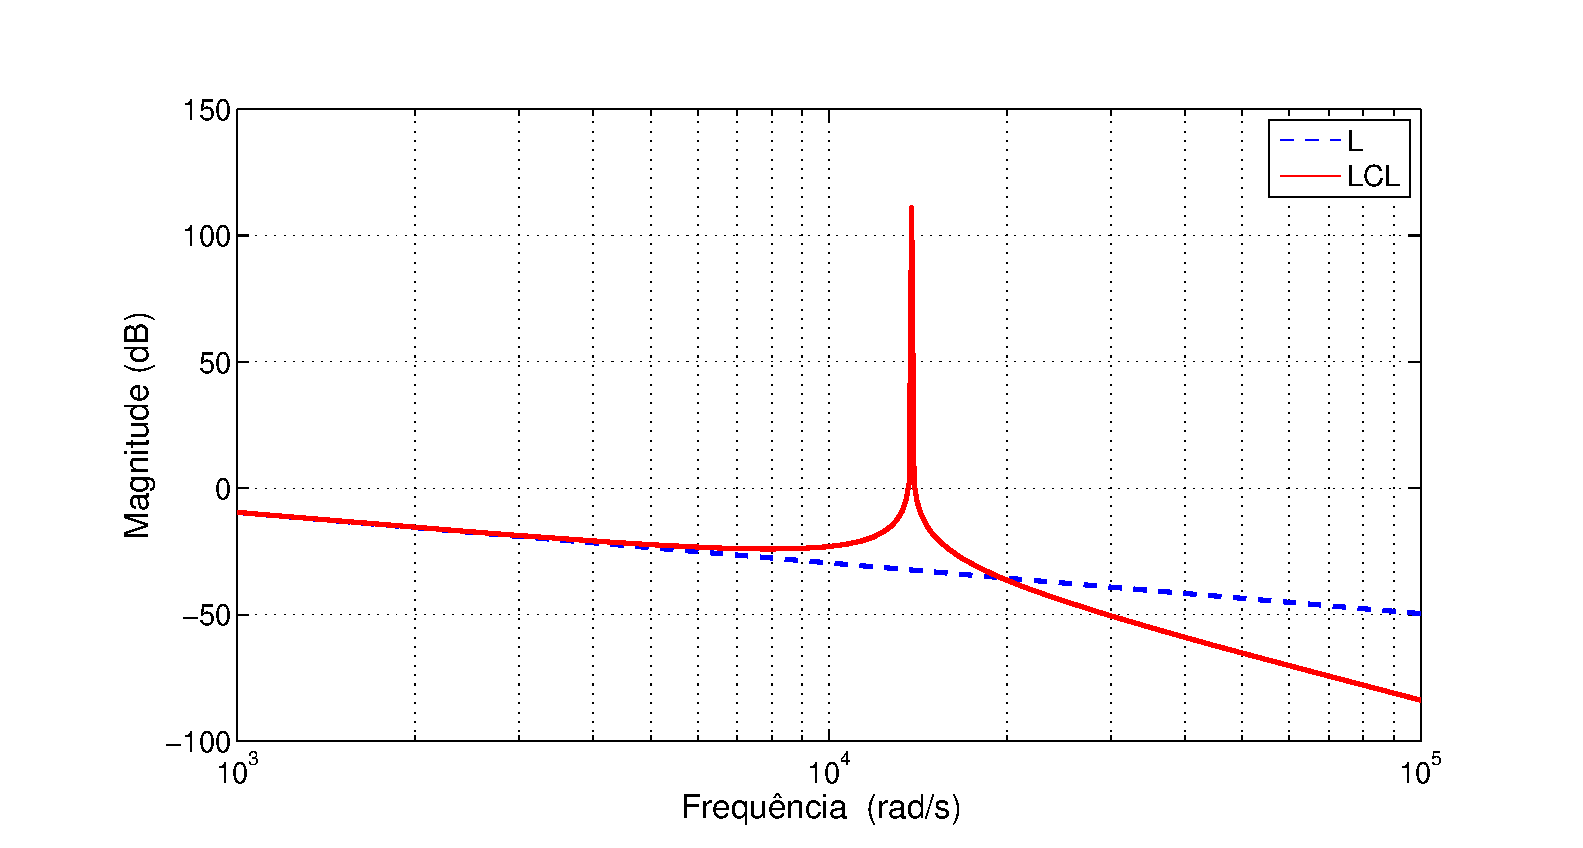
\includegraphics[width=0.9\textwidth]{img/L_vs_LCL}}
    %            \subcaption{Comparação entre filtro L e filtro LCL.}
    %            \label{fig:L_vs_LCL}
    %        \end{minipage}
    %        \begin{minipage}[b]{1\linewidth}
    %            \centering{
    %            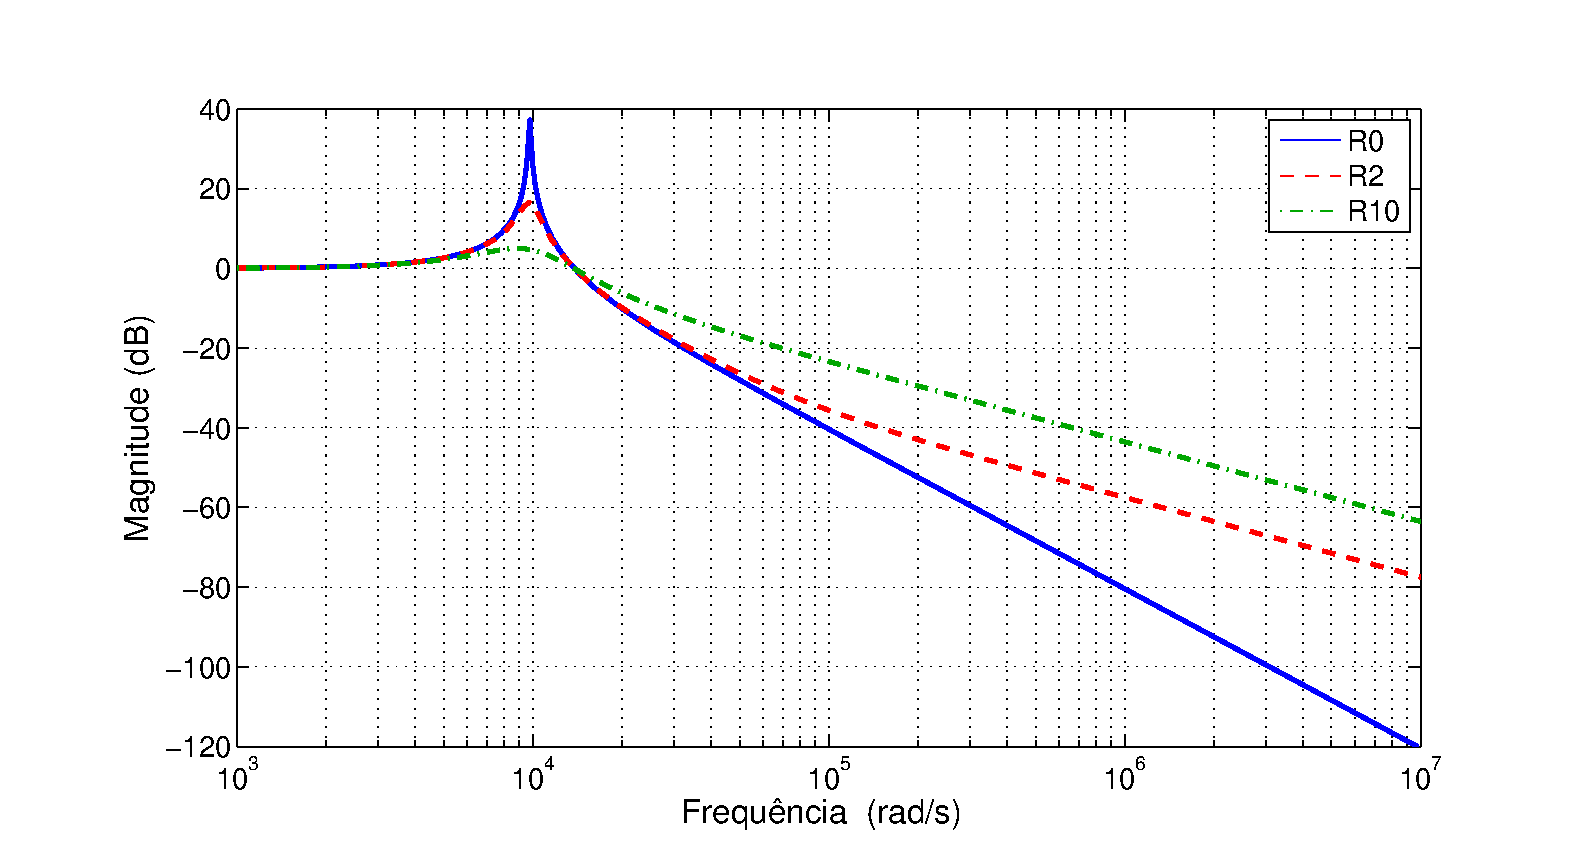
\includegraphics[width=0.9\textwidth]{img/R_in_LCL}}
    %            \subcaption{Efeito do amortecimento passivo.}
    %            \label{fig:R_in_LCL}
    %        \end{minipage}
    %        \renewcommand\figurename{Fig.}
    %        \caption{Diferença entre filtros L, LCL e LCL com amortecimento passivo.}
    %\end{figure}

    \begin{figure}[htb]
        \centering{
            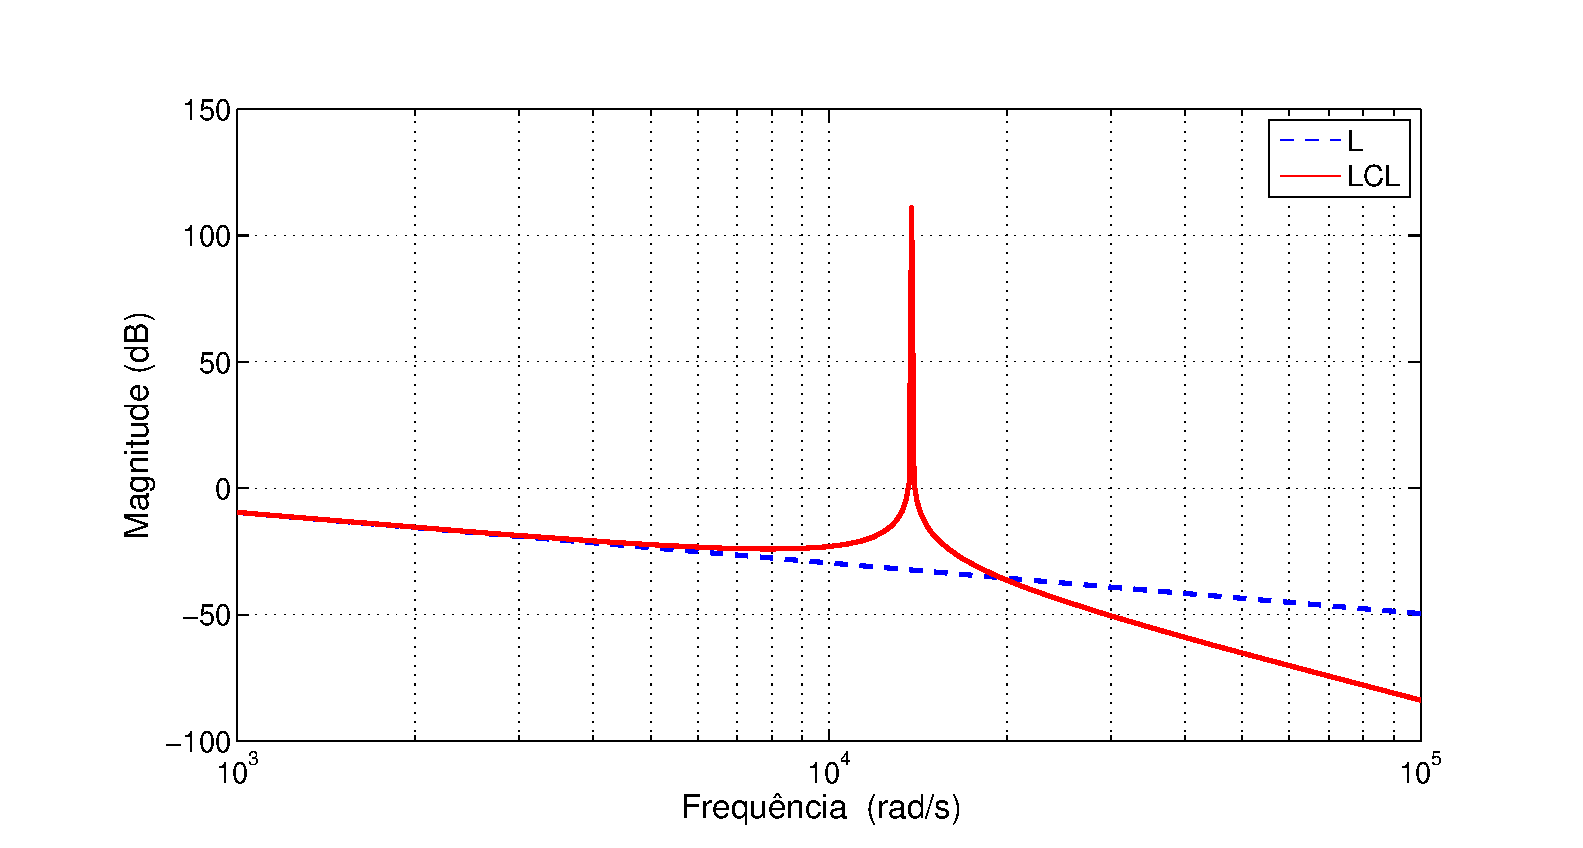
\includegraphics[width=0.9\textwidth]{img/L_vs_LCL}}
        \caption{Comparação entre filtro L e filtro LCL.}
        \label{fig:L_vs_LCL}
    \end{figure}

    A Fig.~\ref{fig:L_vs_LCL} mostra o diagrama de Bode de (\ref{eq:G_v_i2_2})
    com $R_d = 0$ para dois casos: com e sem capacitância $C$. No caso de $C = 0$,
    tem-se o filtro L. No caso de $C \neq 0$, tem-se o filtro LCL.

    Embora nos dois casos a indutância total tenha sido mantida a mesma, observa-se
    que o filtro LCL apresenta uma maior atenuação das harmônicas de comutação
    de alta frequência se comparado ao filtro L. Em contrapartida, o filtro LCL
    possui um pico de amplitude na frequência de ressonância. Por isso, é preciso
    mais cuidado no projeto para manter a estabilidade do sistema.

    O recurso mais comumente utilizado para tal é a adição de um resistor de
    amortecimento $R_d$. O amortecimento passivo, no entanto, reduz a atenuação
    das harmônicas de alta frequência. A Fig.~\ref{fig:R_in_LCL} mostra o diagrama
    de Bode de (\ref{eq:G_i1_i2}) para $R_d = 0$, $R_d = 2$ e $R_d = 10$.

    \begin{figure}[htb]
        \centering{
            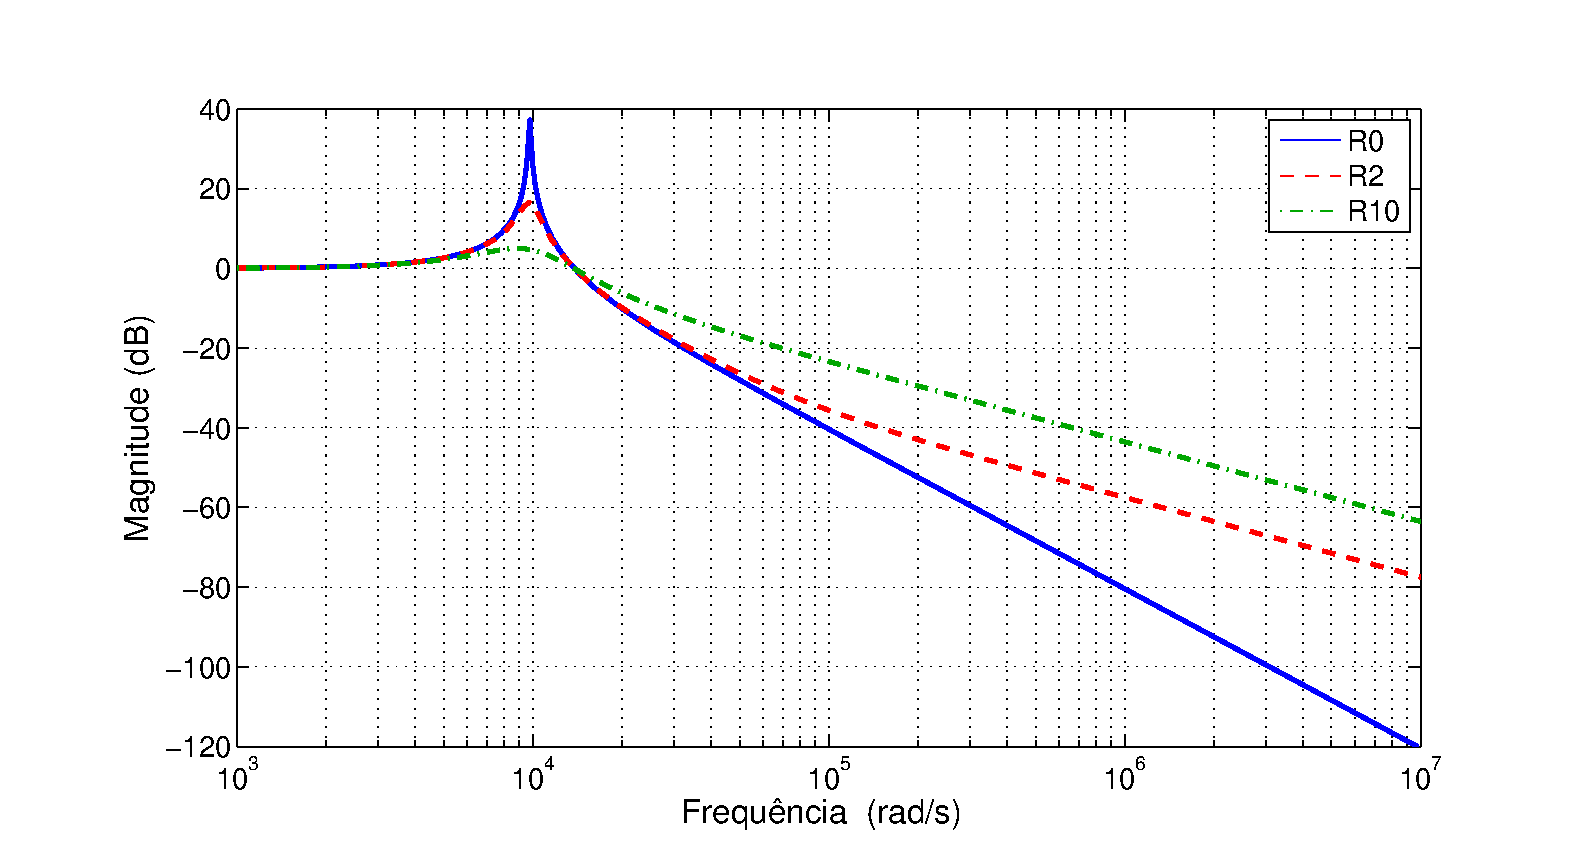
\includegraphics[width=0.9\textwidth]{img/R_in_LCL}}
        \caption{Diferença entre filtros L, LCL e LCL com amortecimento passivo.}
        \label{fig:R_in_LCL}
    \end{figure}

    A redução no amortecimento de harmônicas de alta frequência faz com que filtros
    LCL com amortecimento passivo sejam maiores que filtros LCL sem amortecimento
    passivo, para que atinjam o mesmo desempenho. Esse aumento de tamanho implica
    em aumento de custo e redução da banda passante do filtro.

    As considerações aqui feitas demonstram o porquê da escolha do filtro LCL sem
    amortecimento passivo. Embora seja mais trabalhoso e delicado projetá-lo,
    o desempenho é visivelmente melhor.


\section{Corrente e Tensão do Capacitor}

    O sistema formado pelo conversor alimentado por tensão conectado à rede através
    de um filtro \textit{LCL} é um sistema composto por estados que podem ser
    utilizados em uma estrutura multimalha, onde a malha interna pode ser projetada
    para controlar a tensão ou a corrente do capacitor. Independentemente de qual
    variável é escolhida, o conhecimento da indutância $L_1$ e da capacitância $C$
    do filtro facilitam o projeto da malha interna. Deve haver, no entanto, capacidade
    de rejeição de distúrbios.

    %Comentar que independente de se controlar a tensão ou corrente do capacitor,
    %estas variáveis estão associadas a elementos conhecidos (L1 e C)

    O Controle Multimalha, é adequado para melhorar o desempenho
    de sistemas de controle com apenas uma malha em que o distúrbio esteja
    relacionado com a variável manipulada ou quando o elemento de controle final
    exibe um comportamento não-linear~\cite{ref:LEE}.

    A Fig.~\ref{fig:multiloop} mostra a estrutura geral do Controle Multimalha, onde
    $r_1$ é a referência para a malha externa, $r_2$ é a referência para a malha
    interna, $G_p$ é a função de transferência do controlador primário,
    $G_s$ é a função de transferência do controlador secundário, $P_1$ e $P_2$
    são a planta, $d_1$ e $d_2$ são os distúrbios:

    %\comment{
    %Uma forma
    %de fazer isto é controlar ou a corrente ou a tensão do capacitor. O controle
    %de cada parâmetro tem vantagens sobre o controle do outro, e é necessária
    %uma análise mais aprofundada para verificar qual a melhor opção.
    %}

    \begin{figure}[htb]
        \centering{
            \includegraphics[width=0.9\textwidth]{img/multiloop_geral}}
        \renewcommand\figurename{Fig.}
        \caption{Estrutura geral de Controle Multimalha.}
        \label{fig:multiloop}
    \end{figure}

    A decisão sobre qual variável deve ser controlada em cada uma das malhas é complexa,
    e uma análise mais profunda deve ser feita para verificar qual a melhor
    opção para cada malha. Essa análise é feita em~\cite{ref:NASER}, utilizando o
    método do lugar das raízes e a técnica do espaço de estados médio. Esta é uma técnica
    essencial para a análise de circuitos chaveados, pois permite que as técnicas de
    análise de circuitos tradicionais sejam aplicadas à eles.

    O princípio de funcionamento é que a comutação ciclo à ciclo é ignorada em
    favor das características médias do circuito nas frequências abaixo da
    frequência de Nyquist. Perde-se então a capacidade de ver a forma de onda
    da comutação, mas pode-se determinar rapidamente uma série de fatores
    do circuito, como estabilidade, margem de ganho e de fase, o lugar das
    raízes e a resposta transiente média. Os passos para usar esta técnica são
    os seguintes:

    \begin{enumerate}
        \item Desenhar o circuito em cada estado;
        \item Escrever a equação de nó, malha ou elemento para cada estado;
        \item Determinar qual parcela do período o sistema permanece em cada estado;
        \item Multiplicar cada equação de estado por sua parcela de tempo e somá-las
            para obter uma média ponderada das equações de estado.
    \end{enumerate}

    As funções de transferência da tensão $v_c$ e da corrente $i_c$ do
    capacitor são dadas por:

    \begin{equation}
        v_c = \frac{\frac{2V_{DC}}{L_1} \frac{1}{C} \left( s + \frac{R_2}{L_2} \right)}{s^3 + a_2 s^2 + a_1 s + a_0}
        \label{eq:vc}
    \end{equation}

    \begin{equation}
        i_c = \frac{\frac{2V_{DC}}{L_1} s \left( s + \frac{R_2}{L_2} \right)}{s^3 + a_2 s^2 + a_1 s + a_0}
        \label{eq:ic}
    \end{equation}

    Com

    \begin{equation*}
        a_2 = \frac{R_1}{L_1} + \frac{R_2}{L_2}
    \end{equation*}

    \begin{equation*}
        a_1 = \frac{1}{L_1 L_2} \left( R_1 R_2 + \frac{L_1 + L_2}{C} \right)
    \end{equation*}

    \begin{equation*}
        a_0 = \frac{R_1 + R_2}{C L_1 L_2}
    \end{equation*}

    %\comment{
    %\begin{figure}[htb]
    %        \begin{minipage}[b]{1\linewidth}
    %            \centering{
    %            \includegraphics[width=0.9\textwidth]{img/rlocus_vc}}
    %            \subcaption{Lugar das raízes para a tensão do capacitor.}
    %            \label{fig:rlocus_vc}
    %        \end{minipage}
    %        \begin{minipage}[b]{1\linewidth}
    %            \centering{
    %            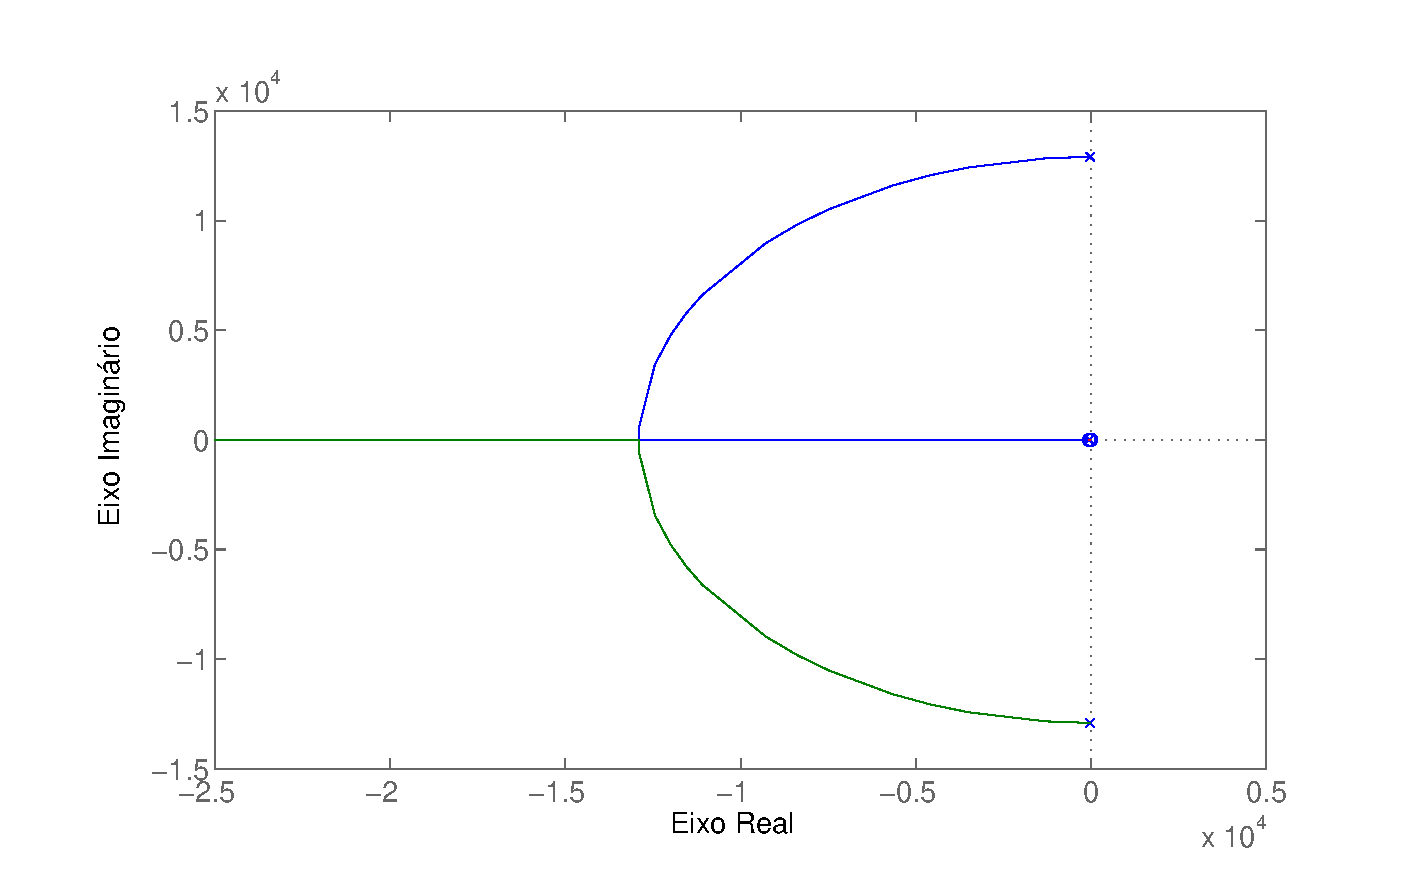
\includegraphics[width=0.9\textwidth]{img/rlocus_ic}}
    %            \subcaption{Lugar das raízes para a corrente do capacitor.}
    %            \label{fig:rlocus_ic}
    %        \end{minipage}
    %        \renewcommand\figurename{Fig.}
    %        \caption{Análise de estabilidade para a corrente e a tensão do capacitor.}
    %\end{figure}
    %}

    A Fig.~\ref{fig:rlocus_vc} mostra o lugar das raízes para a função de
    transferência (\ref{eq:vc}).

    %\comment{
    \begin{figure}[htb]
        \centering{
            \includegraphics[width=0.9\textwidth]{img/rlocus_vc}}
        \renewcommand\figurename{Fig.}
        \caption{Lugar das raízes para a tensão do capacitor.}
        \label{fig:rlocus_vc}
    \end{figure}
    %}

    Percebe-se que os polos da função de transferência da tensão do capacitor
    apresentam um comportamento oscilatório ao longo do eixo imaginário. Devido
    ao projeto do filtro \textit{LCL}, a oscilação não ocorre em uma frequência
    muito alta, o que simplifica o controle desta variável. Além disso, na prática
    haverá sempre parte real nas resistências, o que fará com que os polos desloquem-se
    um pouco para o semiplano esquerdo, saindo do limiar de estabilidade.

    Supondo que o controlador da malha interna tenha um elevado desempenho
    no rastreamento de referências e na rejeição de distúrbios,
    o controle da tensão do capacitor é vantajoso. O capacitor
    pode ser visto como uma fonte de tensão, e toda a dinâmica
    do inversor e do indutor do lado do conversor podem ser ignorados,
    simplificando o controle da corrente da rede.

    A Fig.~\ref{fig:rlocus_ic} mostra o lugar das raízes para a função de
    transferência (\ref{eq:ic}).

    %\comment{
    \begin{figure}[htb]
        \centering{
            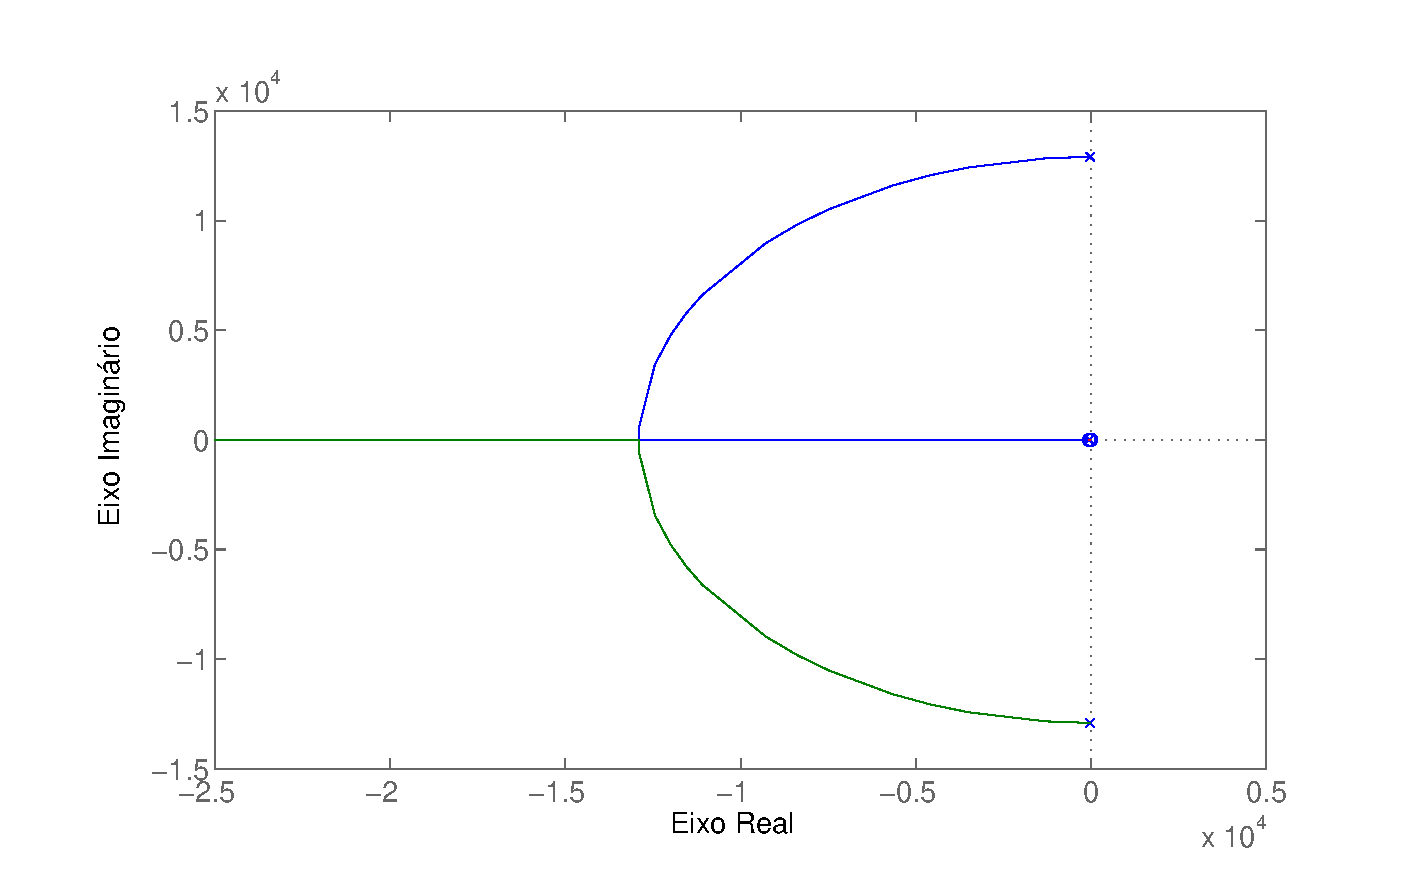
\includegraphics[width=0.9\textwidth]{img/rlocus_ic}}
        \renewcommand\figurename{Fig.}
        \caption{Lugar das raízes para a corrente do capacitor.}
        \label{fig:rlocus_ic}
    \end{figure}
    %}

    Percebe-se que os polos da função de transferência da corrente do capacitor
    deslocam-se para o semiplano esquerdo, indicando que o sistema tende à
    estabilidade. Essa é a grande vantagem de utilizar a corrente do capacitor
    como variável de controle da malha interna.

    A corrente do capacitor mostra-se como uma ótima escolha. No entanto, a tensão
    do capacitor pode ser selecionada como uma variável intermediária a ser controlada,
    sintetizando-se assim uma fonte de tensão controlada por tensão, no caso, o
    conversor. Deste modo, ter-se-á um circuito do tipo \textit{RL} que aproxima o
    comportamento no ponto de conexão.

    Dessa forma, embora a corrente ofereça mais estabilidade, a tensão do capacitor
    é escolhida como variável de controle da malha interna na presença de um controlador
    adaptativo na malha externa, devido ao quanto essa escolha facilita a realização do
    controle da dinâmica do filtro. Outras topologias para a malha externa serão
    avaliadas, e então a corrente do capacitor será utilizada como variável de
    controle para a malha interna.


%FIM---------------------------------------------------------------------------
